%% Public domain image from
%% http://www.public-domain-image.com/objects/computer-chips/slides/six-computers-chips-circuits.html
\renewcommand\chapterillustration{OGL_texture/chapterImage}



\chapter{텍스처(texture)}

\index{텍스처}\index{texture}


텍스처 매핑은 컴퓨터 그래픽스에서 어떤 물체의 표면에 추가적인 재질감이나, 색상 등을 입히는 작업이다. 이러한 텍스처 매핑은 왜 필요한 것일까?
현대의 그래픽 카드는 매우 많은 수의 폴리곤(polygon)을 실시간에 렌더링할 수 있는 능력을 가지고 있다. 하지만, 일상 생활에서 우리가 보는 다양한 물체의 표면을 기하적으로 완벽히 모델링하여 표현하는 것은 아직 불가능한 일이다. 다시 말해 다양한 색상, 다양한 굴곡을 모두 기하적으로 표현할 수 없기에 사용하는 것이 텍스처 매핑이다.

\section{텍스처 매핑의 개념}\index{texture!mapping}\index{텍스처!매핑}\index{매핑!텍스처}

텍스처 매핑(mapping)의 종류는 다양한데, 자주 사용되는 매핑 몇 가지는 다음과 같다.

\begin{itemize}
\item 컬러 매핑: 이미지의 컬러를 표면에 입히는 텍스처 매핑\index{컬러 매핑}\index{매핑!컬러}\index{color mapping}\index{mapping!color}
\item 범프 매핑: 이미지를 활용하여 표면에 굴곡이 있는 것처럼 느끼게 만드는 매핑\index{범프 매핑}\index{매핑!범프}\index{bump mapping}\index{mapping!bump}
\item 환경매핑: 주변의 환경이 객체에 반사되는 형태로 입혀지는 텍스처 매핑\index{환경 매핑}\index{매핑!환경}\index{environment mapping}\index{mapping!environment}
\end{itemize}

각각의 매핑을 통해 얻게 되는 결과는 그림 \ref{fig:OGL_texture:mappings}와 같다.
\begin{figure}[h!]
  \centering
	\begin{tabular}{ccc}
	\fbox{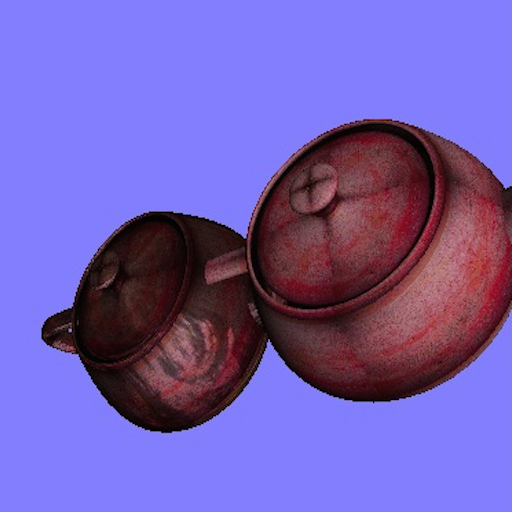
\includegraphics[height=3.5cm]{OGL_texture/mapping_color.png}}&
	\fbox{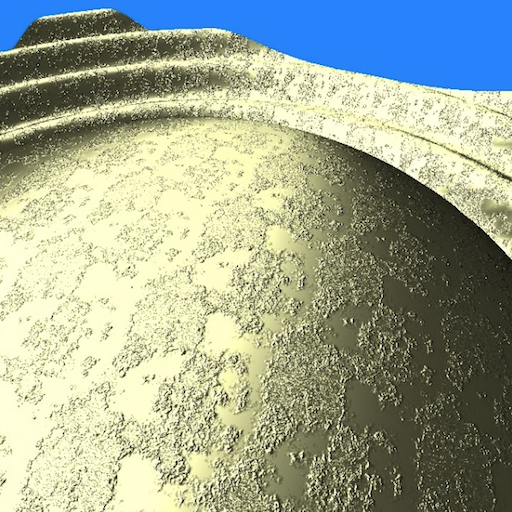
\includegraphics[height=3.5cm]{OGL_texture/mapping_bump.png}}&
	\fbox{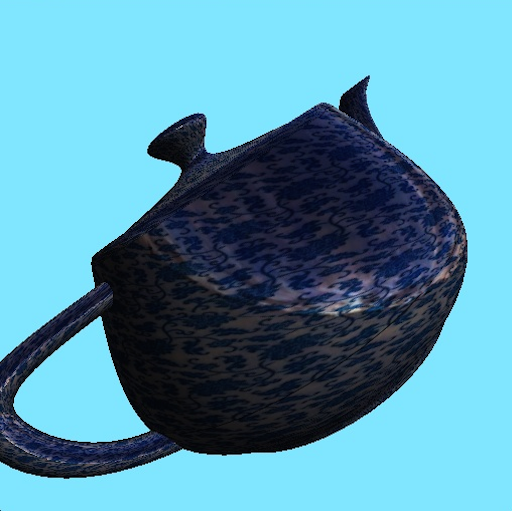
\includegraphics[height=3.5cm]{OGL_texture/mapping_env.png}}\\
(a) 컬러 매핑 & (b) 범프 매핑 & (c) 환경 매핑
\end{tabular}
    \caption{몇 가지 텍스처 매핑의 결과}
    \label{fig:OGL_texture:mappings}
\end{figure}

\subsection{매핑의 기본적인 수학}

텍스처 매핑의 아이디어는 매우 간단하다. 텍스처를 표현하는 이미지의 내용을 물체의 표면으로 옮겨 놓기만 하면 된다. 
이때 텍스처 공간에서의 좌표 $(s,t)$를 텍스처 좌표, 물체 표면의 좌표 $(x,y,z)$를 전역공간 좌표라고 하자.
장면을 표현하는 기하공간의 좌표 (x,y,z)는 실수 원소를 가지는 데에 반해 텍스처 공간의 좌표 (s,t)는 정수 원소를 가진다.
하나의 정수 좌표에 의해 얻어지는 텍스처 이미지 상의 한 점을 텍셀(texel)이라고 부른다. 화면에 그려질 때 화면 좌표계의 한 점을 화소 혹은 픽셀(pixel)이라고
부르는 것처럼 텍스처를 구성하는 기본 요소가 된다. \index{texel}\index{텍셀}


매핑이라는 것은 텍스처가 표현하는 정보를 장면을 표현하는 기하 공간의 물체로 옮기면 되므로, 이것을 이런 매핑 함수로 구현할 수 있다.

$$x = {\mathcal X}(s,t), ~ y = {\mathcal Y}(s,t), ~ z={\mathcal Z}(s,t)$$


\index{전방 매핑}\index{forward mapping}\index{매핑!전방}\index{mapping!forward}
이러한 방식의 매핑을 전방 매핑(forward mapping)이라고 하는데, 여기에는 심각한 문제가 있다. 텍스처 이미지는 정수개의 픽셀로 구성된 데이터이며, 이 유한한 개수의 픽셀을 객체에 옮겨 놓게 되면 빈 공간이 생길 수 있다.

\index{역방향 매핑}\index{backward mapping}\index{매핑!역방향}\index{mapping!backward}
따라서, 실제 텍스처 매핑은 역방향 매핑(backward mapping)을 수행하는데, 다음과 같이 그려지는 물체가 차지하는 화면좌표들마다 전역좌표 (x,y,z)에 해당하는 텍스처 좌표 (s,t)를 구하는 것이다.

$$s = {\mathcal S}(x,y,z), ~ t = {\mathcal T}(x,y,z)$$

이렇게 구해진 $s$와 $t$는 앞서 설명한 텍셀 개념과 달리 매핑 함수에 의해 실수(real number)로 계산될 수도 있다. 
이 경우 어떠한 텍셀을 선택할 것인지는 텍스처 매핑에 적용되는 필터(filter)에 의해 결정된다.
보간을 사용하는 경우에는 실수 값으로 구해진 $(s,t)$와 인접한 네 개의 텍셀을 쌍선형보간(bilinear interpolation)하는 방식을 사용할 수 있으며,
다른 방식으로는 인접한 네 개의 텍셀 가운데 가장 가까운 텍셀을 사용하는 것도 가능하다.
\index{매핑 필터}\index{mapping filter}
\index{쌍선형 보간}\index{bilinear interpolation}

\begin{figure}[h!]
  \centering
	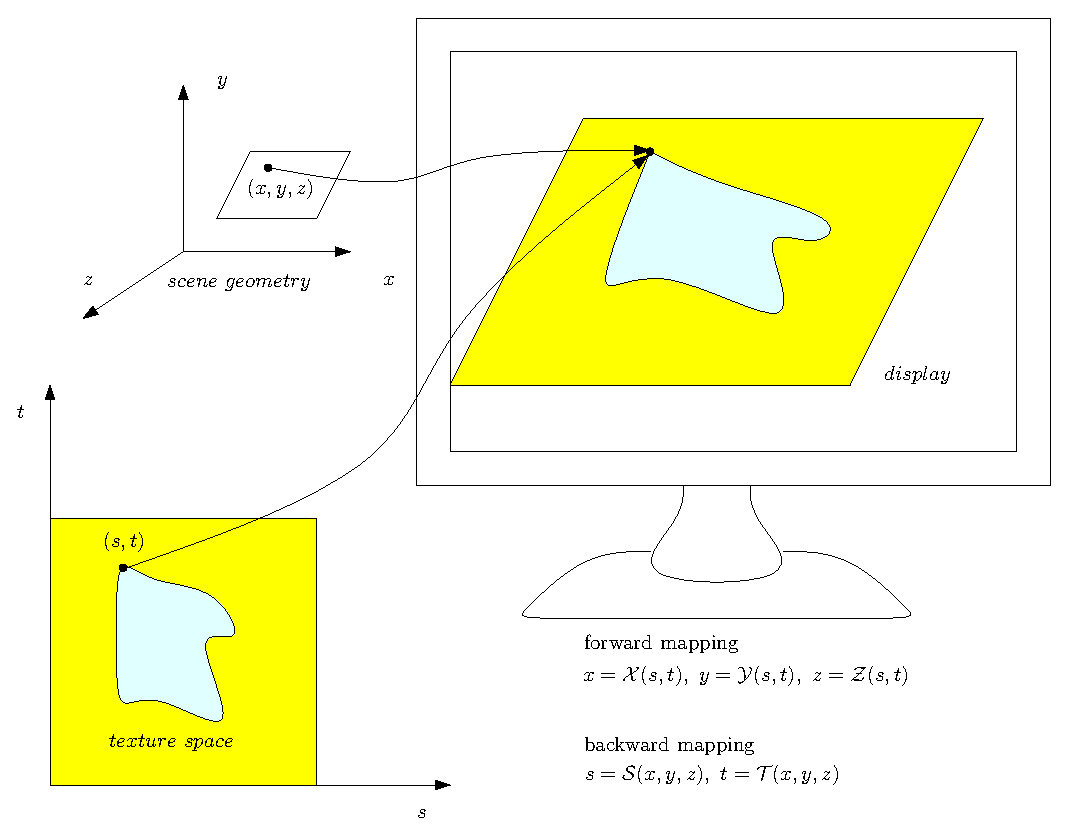
\includegraphics[height=9cm]{OGL_texture/textureMapping.eps}
    \caption{텍스처 매핑에 필요한 좌표 변환 개념}
    \label{fig:OGL_texture:mappingConcept}
\end{figure}

이 두 함수는 어떻게 찾을 수 있을까? 수학적 모델로 이 함수를 구하는 것은 쉽지 않다. 
가장 많이 사용되는 기법은 기하 모델을 결정하는 정점마다 텍스처 좌표를 직접 지정하는 것이다.
텍스처 매핑의 기본적인 좌표 변환 개념은 그림 \ref{fig:OGL_texture:mappingConcept}에 나타나 있다.


\subsection{OpenGL을 이용한 텍스처 매핑 구현}\index{텍스처!오픈지엘 구현}\index{texture!OpenGL implementation}
OpenGL에서 텍스처를 적용하는 과정은 다음과 같은 3 개의 단계를 거친다.
\begin{itemize}
\item {\small \sf 텍스처 지정  - 이미지 읽기 혹은 생성, 텍스처 지정, 텍스처 사용 가능하게 하기}
\item {\small \sf 각 정점에 텍스처 좌표 지정 - 매핑 함수는 응용 프로그램의 몫}
\item{\small \sf 텍스처 파라미터 설정 - 래핑(wrapping), 필터링(filtering) 방법 설정}
\end{itemize}

\index{텍스처!오픈지엘}\index{texture!OpenGL}
앞서 살펴본 바와 같이 텍스처를 적용하기 위해서는 가장 먼저 텍스처를 지정해야 한다. 텍스처를 지정한다는 것은 매핑에 사용할 텍스처를 저장하고 있는 이미지를 읽어 이를 그래픽카드에 있는 텍스처 메모리로 옮기고 사용가능한 텍스처로 만들거나, 절차적(procedural) 방법을 통해 이미지 데이터를 생성한 뒤에 이를 그래픽카드에 있는 텍스처 메모리에 옮기는 방법이다. 우선 작은 배열에 임의로 값을 주어 간단한 이미지를 직접 생성해 보자. 아래의 코드 \ref{code:OGL_texture:simpleProcTexture}는 
16$\times$16 크기의 이미지를 나타내고 있다. 하나의 픽셀은 세 개의 원소 (r,g,b)를 가지고 있다. 각각의 원소에 대해 임의의 값을 설정하고 있는데, 이 값은 0에서 255사이의 값으로 GLubyte 형 데이터이다. 

\begin{algorithmbis}[텍스처 이미지 데이터 생성하기]\label{code:OGL_texture:simpleProcTexture}
\lstset{language=C++, escapechar=^} 
\begin{lstlisting}
GLubyte myTex[TEXSIZE][TEXSIZE][3];  // ^{\it {\sf TEXSIZE}는 16으로 정의된 것으로 가정하자}^
void CreateTexture(void) {
  for(int i=0;i<TEXSIZE;i++) {
    for(int j=0;j<TEXSIZE;j++) {
       for(int k=0;k<3;k++) {			
          myTex[i][j][k] = (GLubyte) (255*float(rand()\%1000)/999.0);
       } // end k
    } // end j
  } // end i
}
\end{lstlisting}
\end{algorithmbis}

이렇게 만들어진 배열은 이미지를 담고 있을뿐 오픈지엘이 사용할 수 있는 텍스처가 아니다. 이를 오픈지엘에서 활용할 수 있는 텍스처로 만드는 방법은 {\sf glTexImage2D} 같은 함수를 사용하는 것이다.
다음의 코드 \ref{code:OGL_texture:openglTexture}는 {\sf glTexImage2D}를 이용하여 앞서 준비한 배열(이미지)를 오픈지엘 텍스처로 만드는 작업을 수행한다. 오픈지엘은 가능한 최소의 작업을 수행하려 노력하기 때문에 기본적으로 텍스처 매핑은 사용하지 않는 상태로 설정되어 있다. 이를 변경하여 텍스처 매핑을 수행하도록 하여야 하며, 텍스처 매핑을 수행할 때 어떠한 방식으로 적용할 것인지를 설정한다. 다음 코드는 이러한 과정이 정리되어 있다.

\begin{algorithmbis}[오픈지엘 텍스처 생성]\label{code:OGL_texture:openglTexture}
\lstset{language=C++} 
\begin{lstlisting}
void SetupTexture(void) 
{
  glTexImage2D(GL_TEXTURE_2D, 0, GL_RGB, 
            TEXSIZE, TEXSIZE, 0, GL_RGB, 
            GL_UNSIGNED_BYTE, &myTex[0][0][0]);
	
  glTexParameterf(GL_TEXTURE_2D, GL_TEXTURE_WRAP_S, GL_CLAMP);
  glTexParameterf(GL_TEXTURE_2D, GL_TEXTURE_WRAP_T, GL_REPEAT);
  glTexParameterf(GL_TEXTURE_2D, GL_TEXTURE_MAG_FILTER, GL_LINEAR);
  glTexParameterf(GL_TEXTURE_2D, GL_TEXTURE_MIN_FILTER, GL_NEAREST);
  glEnable(GL_TEXTURE_2D);
}
\end{lstlisting}
\end{algorithmbis}

위의 코드에서 가장 먼저 나오는 {\sf glTexImage2D}는 2차원 텍스처 ({\sf GL\_TEXTURE\_2D})를 생성하는 것으로 앞서 만든 {\sf myTex} 배열의 이미지를 활용한다. 크기가 {\sf TEXSIZE} $\times$ {\sf TEXSIZE}이므로 이 크기를 지정하고 있으며, 각각의 원소가 {\sf GL\_UNSIGNED\_BYTE}임도 알려주고 있다. 그리고 이미지의 내용은 
{\sf GL\_RGB} 모드로 저장되어 있음도 함께 설정하고 있다.
그 뒤에 이어지는 코드는 텍스처 좌표 $s$와 $t$가 [0,1]의 범위를 넘어설 때에 어떻게 할 것인지를 지정한다. 
{\sf GL\_CLAMP}는 0보다 작거나, 1보다 큰 경우, 각각 0와 1로 취급한다. 1을 넘을 경우 다시 0에서 시작하게 하는 방식은 {\sf GL\_WRAP}이다.
그 다음 나타나는 {\sf MAG/MIN} 필터는 텍스처가 원래의 크기보다 더 큰 공간으로 가거나, 더 작은 공간으로 갈 때, 보간을 수행하거나({\sf GL\_LINEAR}), 가장 가까운 텍셀을 사용하는({\sf GL\_NEAREST}) 방식을 결정한다.

마지막으로 {\sf GL\_TEXTURE\_2D}를 사용할 수 있도록 glEnable 함수를 이용하여 상태 변경을 한다. 이제 텍스처 매핑을 사용할 수 있게 되었다.
그림을 그리는 것은 다음 코드 \ref{code:OGL_texture:textureCoord}과 같이 각각의 정점에 텍스처 좌표 $(s,t)$를 지정한다. 
이렇게 정점별로 텍스처 좌표가 지정되면, 폴리곤 내부의 점들의 텍스처 좌표는 선형보간을 통해 결정된다.
이 코드를 실행하면 그림 \ref{fig:OGL_texture:texMap1}과 같은 결과를 얻게 된다. 이는 우리가 랜덤 함수를 통해 생성한 이미지이다.

\begin{algorithmbis}[텍스처 좌표를 지정하여 사각형 그리기]\label{code:OGL_texture:textureCoord}
\lstset{language=C++} 
\begin{lstlisting}
void drawAPlane(void) {
  float m=-1;
  float p= 1;
  glBegin(GL_QUADS);
   glTexCoord2f(0, 1);
   glVertex3f(m,p,0); 
   glTexCoord2f(0, 0);
   glVertex3f(m,m,0); 
   glTexCoord2f(1, 0);
   glVertex3f(p,m,0); 
   glTexCoord2f(1, 1);
   glVertex3f(p,p,0);
  glEnd();
}
\end{lstlisting}
\end{algorithmbis}


\begin{figure}[h!]
  \centering
	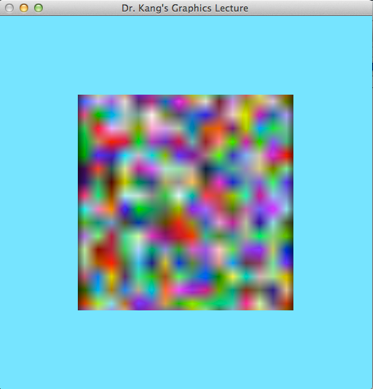
\includegraphics[height=6cm]{OGL_texture/texMap1.png}
    \caption{각 픽셀에 임의의 색이 칠해진 16$\times$16 이미지를 매핑한 결과}
    \label{fig:OGL_texture:texMap1}
\end{figure}

이때 이 이미지가 흐리게 나타나는 이유는 {\sf GL\_TEXTURE\_MAG\_FILTER}를 {\sf GL\_LINEAR}로 
설정했기 때문인데, 이를 {\sf GL\_NEAREST}로 바꾸면 텍셀 값을 보간하지 않고 가장 가까운 값을 그대로 가지고 오기 때문에
다음 그림 \ref{fig:OGL_texture:texMap2}과 같이 원래의 이미지를 또렷하게 확대한 장면을 얻는다.

\begin{figure}[h!]
  \centering
	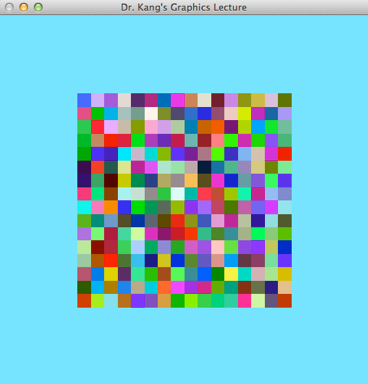
\includegraphics[height=6cm]{OGL_texture/texMap2.png}
    \caption{GL\_NEAREST 필터로 16$\times$16 이미지를 매핑한 결과}
    \label{fig:OGL_texture:texMap2}
\end{figure}

텍스처를 사용한 상태에서 {\sf glutSolidTeapot(...)}을 호출하면 다음 그림 \ref{fig:OGL_texture:texMap3}과 같이 그려진다. 이때 앞서 다룬 조명을 제대로 설정해야 주전자가 음영을 갖고 그려진다.

\begin{figure}[h!]
  \centering
	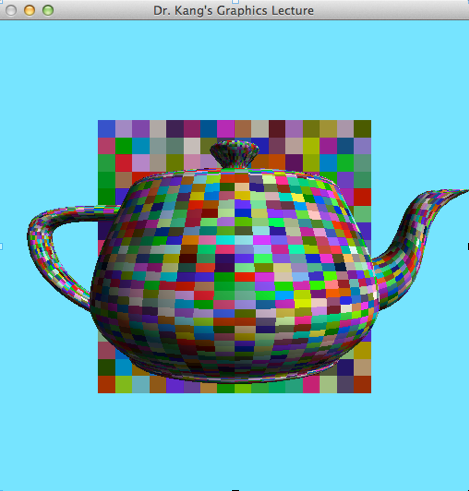
\includegraphics[height=6cm]{OGL_texture/texMap3.png}
    \caption{glutSolidTeapot으로 그려진 주전자에 매핑된 이미지}
    \label{fig:OGL_texture:texMap3}
\end{figure}


\subsection{이미지 파일을 읽어 텍스처로 사용하기}

이미지 파일을 직접 절차적으로 생성하는 방식은 다양한 텍스처를 손쉽게 만들 수 있는 방법은 아니다. 좀 더 효율적인 방법은 이미지 편집 도구를 이용하여 텍스처 이미지를 만들고, 이를 불러서 사용하는 것이다. 이를 위해서는 이미지 파일을 다루는 코드를 작성해야 한다. 우리는 이를 직접 작성하지 않고, 이미 만들어져 공개된 소스를 활용할 것이다.
우선 응용 프로그램의 소스에서 텍스처를 설정하는 작업을 진행해야 한다. 이미지를 읽어들이는 방법은 STB Image 라이브러리를 사용할 것이며, 이 라이브러리는 다음 URL에서 구할 수 있다. 이 라이브러리는 소스코드를 그대로 활용할 수 있다.
\begin{verbatim}
http://www.nothings.org/stb_image.c
\end{verbatim}
이 책과 함께 제공되는 소스코드 데이터를 보면 이 파일을 헤더와 소스로 구분하여 각각 {\sf STBImage.h}와 {\sf STBImage.cpp}로 저장해 둔 것을 확인할 수 있을 것이다. 이 라이브러리를 이용하면 다음과 같이 간단하게 이미지를 읽어 배열에 저장할 수 있으며, 오픈지엘 코드에서 쉽게 활용할 수 있다. 다음 코드 \ref{code:OGL_texture:imgLoad}은 그 예이다.


\begin{algorithmbis}[STB Image 라이브러리로 이미지 읽어 들이기]\label{code:OGL_texture:imgLoad}
\lstset{language=C++} 
\begin{lstlisting}
int width, height, bitsPerPixel;
unsigned char *data = stbi_load("cosmos.jpg", &width, &height, &bitsPerPixel, 0);
glGenTextures(1, &texture);
glBindTexture(GL_TEXTURE_2D, texture);
glTexImage2D(GL_TEXTURE_2D, 0, GL_RGB, 
			width, height, 0, GL_RGB, GL_UNSIGNED_BYTE, data);
\end{lstlisting}
\end{algorithmbis}

프로젝트에서 활용할 텍스처를 준비하고 그 이름을 {\sf cosmos.jpg}라고 하자. 텍스처에 사용할 이미지를 읽고 이를 OpenGL 텍스처로 만드는 코드는 {\sf texture.h}와 
{\sf texture.cpp}에서 구현한다.  앞서 설명한 STB 이미지 라이브러리를 이용하여 각각의 소스 코드를 다음 코드 \ref{code:OGL_texture:imgTexture}과 
같이 작성할 수 있다.

\begin{algorithmbis}[이미지 읽어 텍스처 만들기]\label{code:OGL_texture:imgTexture}
\lstset{language=C++, escapechar=^} 
\begin{lstlisting}
^{\sf \color{red} texture.h}^
...
GLuint setTexture(char *filename);
...


^{\sf \color{red} texture.cpp}^
...
#include "STBImage.h"
GLuint setTexture(char *filename) {
	GLuint texture;
	int width, height, bitsPerPixel;
	unsigned char *data = stbi_load(filename, &width, &height, &bitsPerPixel, 0);
	glGenTextures(1, &texture);
	glBindTexture(GL_TEXTURE_2D, texture);
	glTexImage2D(GL_TEXTURE_2D, 0, GL_RGB,
				width, height, 0, GL_RGB, GL_UNSIGNED_BYTE, data);

	glTexParameterf(GL_TEXTURE_2D, 		GL_TEXTURE_WRAP_S, GL_REPEAT);
	glTexParameterf(GL_TEXTURE_2D, 		GL_TEXTURE_WRAP_T, GL_REPEAT);
	glTexParameterf(GL_TEXTURE_2D, 		GL_TEXTURE_MAG_FILTER, GL_LINEAR);
	glTexParameterf(GL_TEXTURE_2D, 		GL_TEXTURE_MIN_FILTER, GL_LINEAR);
	glEnable(GL_TEXTURE_2D);
	return texture;
}
\end{lstlisting}
\end{algorithmbis}

OpenGL 응용 프로그램에서 텍스처가 준비되면 이 텍스처는 앞서 임의로 만든 배열처럼 텍스처로 사용할 수 있다. 
{\sf setTexture} 함수는 이미지를 읽어 들여 OpenGL이 사용할 수 있는 배열로 만들어 주는 것이다.
우선 {\sf baboon.jpg}라는 이미지 파일을 준비하여, 프로젝트가 읽을 수 있는 위치에 두자.
{\sf main.cpp}를 다음과 같이 고치면 이 파일을 읽어 텍스처 매핑을 수행할 수 있다.
그 결과는 그림 \ref{fig:OGL_texture:textureImageApplied}에 나타나 있다.

\begin{algorithmbis}[텍스처 적용하기]\label{code:OGL_texture:TextureApplication}
\lstset{language=C++} 
\begin{lstlisting}
void display() {
  glClear(GL_COLOR_BUFFER_BIT|GL_DEPTH_BUFFER_BIT);
  glMatrixMode(GL_MODELVIEW);
  glLoadIdentity();
  gluLookAt(0, 0, 3, 0, 0, 0, 0, 1, 0);
  LightPositioning();
  drawAPlane();
  glutSolidTeapot(1.0);
  glutSwapBuffers();
}
\end{lstlisting}
\end{algorithmbis}


\begin{figure}[h!]
  \centering
	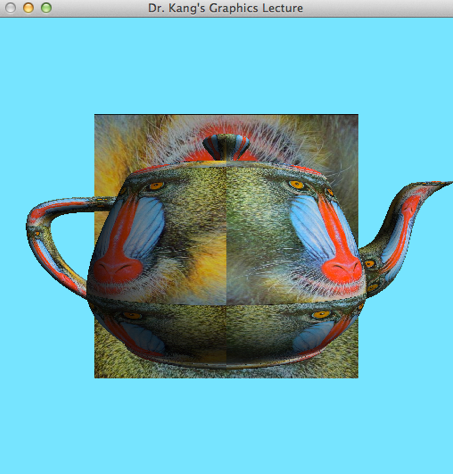
\includegraphics[height=10cm]{OGL_texture/textureImageApplied.png}
    \caption{glutSolidTeapot으로 그려진 주전자에 매핑된 이미지}
    \label{fig:OGL_texture:textureImageApplied}
\end{figure}

\subsection{복수의 텍스처 사용 - 텍스처 바인딩(binding)}
\index{텍스처 바인딩}\index{texture binding}

지금까지는 하나의 텍스처를 사용하였다. 이제 복수의 텍스처를 사용하는 방법에 대해 살펴볼 것이다. 이를 위해서는 두 개의 텍스처를 다룰 수 있도록 텍스처를 가리키는 번호를 저장할 두 개의 변수가 필요하며, 각각의 텍스처를 사용해야 할 때마다, 원하는 텍스처를 지정하는 작업이 필요하다.
이를 텍스처 바인딩(texture binding)이라고 부른다.
우선 두 개의 텍스처를 읽어 들여, 각각을 서로 다른 변수로 관리하는 방법은 다음 코드 \ref{code:OGL_texture:multTextures}과 같다.
그리고 두 개의 텍스처를 필요에 따라 사용가능한 텍스처로 바인딩(binding)하여 사용되는 텍스처를 결정할 수 있다.
그러면 그림 \ref{fig:OGL_texture:multipleTextures}과 같이 평면과 주전자에 다른 텍스처가 적용된다.

\index{텍스처!복수 텍스처 사용}\index{texture!multiple textures}
\index{복수의 텍스처}\index{multiple textures}
\begin{algorithmbis}[복수의 텍스처 읽어 들이기]\label{code:OGL_texture:multTextures}
\lstset{language=C++} 
\begin{lstlisting}
  GLuint tex1, tex2;
  tex1 = setTexture("baboon.jpg");
  tex2 = setTexture("cartoon.jpg");
  glBindTexture(GL_TEXTURE_2D, tex1);
  drawAPlane();
  glBindTexture(GL_TEXTURE_2D, tex2);
  glutSolidTeapot(0.75);
\end{lstlisting}
\end{algorithmbis}

\begin{figure}[h!]
  \centering
	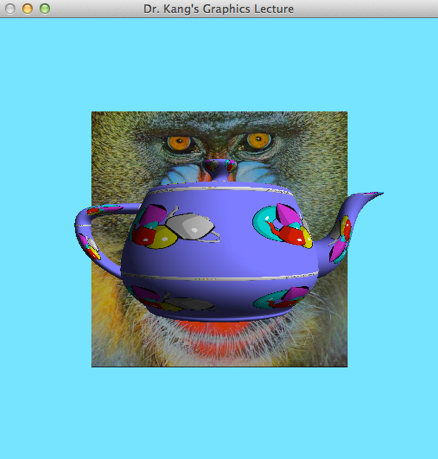
\includegraphics[height=5cm]{OGL_texture/multipleTextures.png}
    \caption{서로 다른 텍스처가 매핑된 두 개의 객체}
    \label{fig:OGL_texture:multipleTextures}
\end{figure}

\section{텍스처 좌표 자동 생성}
\index{texture!automatic texture coordinate}
\index{텍스처!텍스처 좌표 자동 생성}
\index{automatic texture coordinate}
\index{텍스처 좌표 자동 생성}

앞서 우리가 다룬 텍스처 매핑은 정점 데이터의 텍스처 좌표를 일일이 지정하는 방식이다. 그런데, 텍스처 좌표를 자동으로 생성할 수 있다면, 일일히 텍스처 좌표를 지정하지 않고 생성 방법에 따라 알고리즘적으로 적용하거나, OpenGL에게 맡길 수 있다. 특히 환경 매핑과 같은 경우에 이 기법이 유용하게 사용될 수 있다.
이 절에서는 OpenGL이 자동으로 각 정점의 텍스처 좌표를 결정하는 방법을 살펴 볼 것이다. 이 방법을 사용하면, 일일이 정점마다 텍스처 좌표를 줄 필요가 없다.
자동 텍스처 좌표 생성 활성화
텍스처 좌표를 자동으로 생성할 때, $S$와 $T$ 좌표 가운데 어떤 좌표를 자동으로 생성할 것인지를 결정할 수 있다. 다음 코드 \ref{code:OGL_texture:autoTexCoord}은 
두 좌표 모두 자동으로 생성함을 의미한다.


\begin{algorithmbis}[텍스처 좌표 자동 생성 모드 활성화]\label{code:OGL_texture:autoTexCoord}
\lstset{language=C++} 
\begin{lstlisting}
glEnable(GL_TEXTURE_GEN_S);
glEnable(GL_TEXTURE_GEN_T);
\end{lstlisting}
\end{algorithmbis}



\subsection{텍스처 좌표 생성 모드 결정}
\index{texture!GL\_EYE\_LINEAR}
\index{GL\_EYE\_LINEAR}


이제 텍스처 좌표를 실제로 생성하는 방식을 결정한다. 이때는 다음과 같은 코드 \ref{code:OGL_texture:TexEyeLinear}를 사용한다.


\begin{algorithmbis}[GL\_EYE\_LINEAR 방식으로 텍스처 좌표 자동 생성]\label{code:OGL_texture:TexEyeLinear}
\lstset{language=C++} 
\begin{lstlisting}
glTexGenf(GL_S, GL_TEXTURE_GEN_MODE, 	GL_EYE_LINEAR);
glTexGenf(GL_T, GL_TEXTURE_GEN_MODE, 	GL_EYE_LINEAR);
\end{lstlisting}
\end{algorithmbis}


이 코드는 텍스처 좌표 $S$와 $T$ 모두에 대해 자동생성 방식을 {\sf GL\_EYE\_LINEAR} 방식으로 하라는 것이다. 
주전자를 이러한 방식으로 그리면 다음 그림 \ref{fig:OGL_texture:eyeLinear}과 같은 결과가 나온다


\begin{figure}[h!]
  \centering
	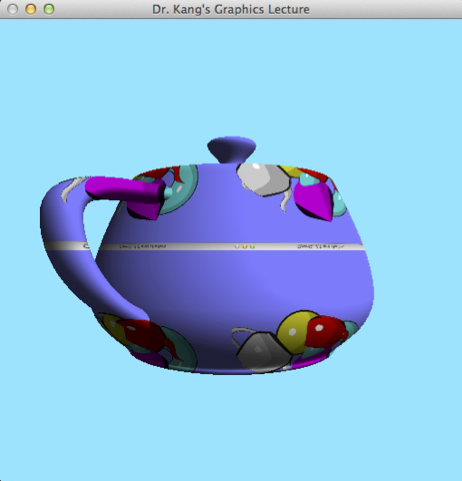
\includegraphics[height=6cm]{OGL_texture/eyeLinear1.png}
	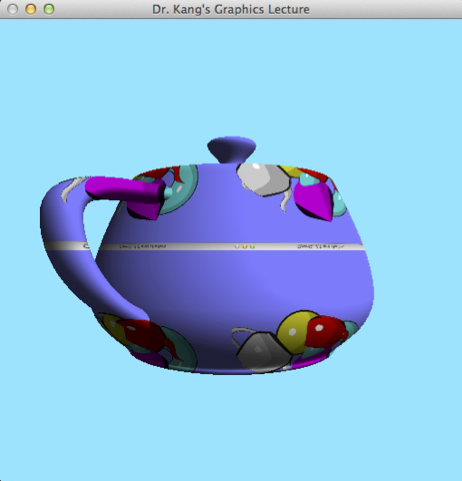
\includegraphics[height=6cm]{OGL_texture/eyeLinear2.png}
    \caption{{\sf GL\_EYE\_LINEAR} 방식으로 생성한 텍스처 좌표로 매핑한 결과}
    \label{fig:OGL_texture:eyeLinear}
\end{figure}

그림에서 확인할 수 있는 바와 같이 물체의 위치에 관계 없이, 눈의 위치와 시선 방향을 기준으로 텍스처가 입혀진다.
이를 다음과 같이 {\sf GL\_OBJECT\_LINEAR}로 변경하면 다음 그림 \ref{fig:OGL_texture:objLinear}과 같은 모습을 보인다.
\index{texture!GL\_OBJECT\_LINEAR}
\index{GL\_OBJECT\_LINEAR}

\begin{figure}[h!]
  \centering
	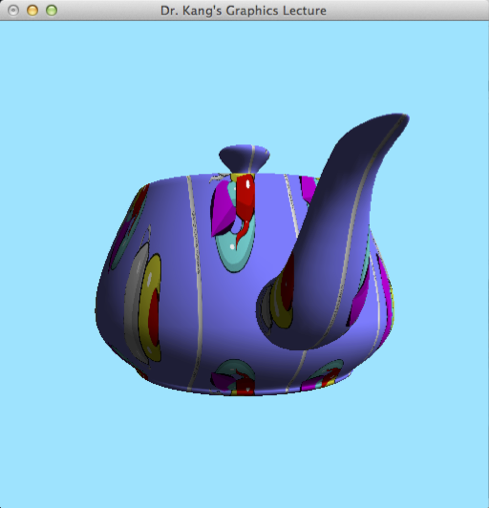
\includegraphics[height=6cm]{OGL_texture/objLinear1.png}
	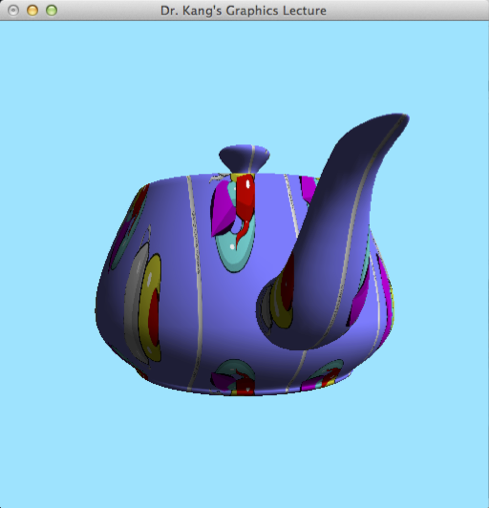
\includegraphics[height=6cm]{OGL_texture/objLinear2.png}
    \caption{{\sf GL\_OBJECT\_LINEAR} 방식으로 생성한 텍스처 좌표로 매핑한 결과}
    \label{fig:OGL_texture:objLinear}
\end{figure}

{\sf GL\_EYE\_LINEAR}가 객체의 표면에 부착되지 않고 프로젝터로 투영한 것과 같은 느낌이라면, 
{\sf GL\_OBJECT\_LINEAR}는 객체 공간에서 입혀진 것이기 때문에 객체가 움직여도 표면에 잘 부착되어 있다. 

또 다른 방법으로 구면 매핑 기법이 있다. 이 기법은 환경 매핑을 할 때 흔히 사용되는 기법이다. 이 방식에서 텍스처 좌표를 결정하는 방법은 시선 벡터를 기준으로 정렬했을 때, 각 정점의 법선 벡터가 가리키는 방향이 텍스처 좌표가 되는 것이다.  실제 코딩은 다음 코드 \ref{code:OGL_texture:SphereMap}과 같다.

\index{texture!GL\_SPHEREMAP}
\index{GL\_SPHEREMAP}
\begin{algorithmbis}[구면 매핑(sphere mapping)의 적용]\label{code:OGL_texture:SphereMap}
\lstset{language=C++} 
\begin{lstlisting}
glTexGenf(GL_S, GL_TEXTURE_GEN_MODE, GL_SPHERE_MAP);
glTexGenf(GL_T, GL_TEXTURE_GEN_MODE, GL_SPHERE_MAP);
\end{lstlisting}
\end{algorithmbis}

이 방법은 특별한 텍스처와 같이 함께 사용될 때에 가장 효과적인데, 이 특별한 텍스처를 구면 맵(sphere map)이라고 한다.
구면 맵의 예는 그림 \ref{fig:OGL_texture:sphereMap} (a)와 같은 것들이다. 
이 텍스처는 구에 비친 환경을 보여준다. 어떤 정점을 카메라에서 쳐다 보자. 법선 벡터의 시작 지점은 텍스처의 중심인 (0.5, 0.5)의 위치에 있다고 하자. 그러면 법선 벡터의 끝 점은 위의 텍스처 이미지 가운데 원형으로 나타난 그림 위의 어딘가에 놓일 것이고, 이 지점의 좌표를 텍스처 좌표로 본다. 이때 법선 벡터의 길이를 반으로 줄여서 위의 텍스처 중심에 놓는 것으로 보면 된다.

\begin{figure}[h!]
  \centering
	\begin{tabular}{cc}\\ \hline
	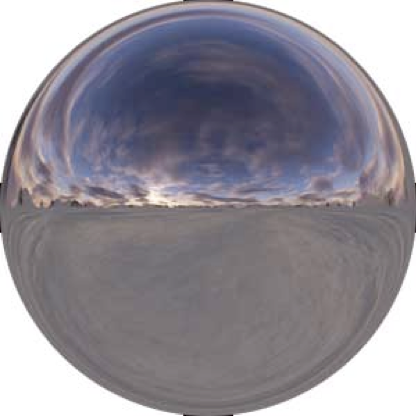
\includegraphics[height=6cm]{OGL_texture/sphereMap.png} &
	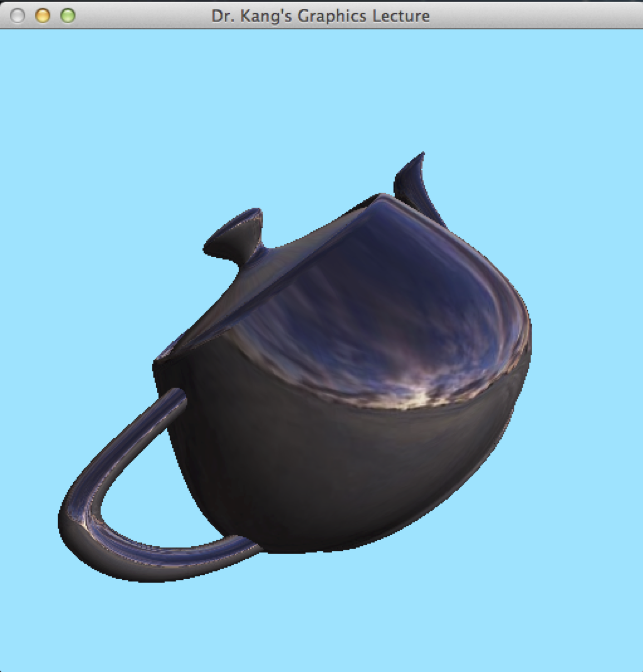
\includegraphics[height=6cm]{OGL_texture/sphereMapped.png} \\
	(a) 구면 맵의 예 & (b) 구면 맵이 적용된 결과
	\end{tabular}
    \caption{구면 맵(sphere map)의 예와 적용 결과}
    \label{fig:OGL_texture:sphereMap}
\end{figure}

그림 \ref{fig:OGL_texture:sphereMap}의 텍스처를 적용했을 때, 주전자는 다음 그림 \ref{fig:OGL_texture:sphereMap} (b)와 같이 그려진다.

이상의 매핑을 모두 모아서 다음 코드 \ref{code:OGL_texture:autoMappings}과 같이 비교할 수 있다.

\begin{algorithmbis}[각종 텍스처 좌표 자동 생성의 비교]\label{code:OGL_texture:autoMappings}
\lstset{language=C++} 
\begin{lstlisting}
	glTranslated(-0.5, 0.0, 0.0);
	glBindTexture(GL_TEXTURE_2D, tex1);
	glEnable(GL_TEXTURE_GEN_S); glEnable(GL_TEXTURE_GEN_T);
	glTexGenf(GL_S, GL_TEXTURE_GEN_MODE, 	GL_EYE_LINEAR);
	glTexGenf(GL_T, GL_TEXTURE_GEN_MODE, 	GL_EYE_LINEAR);
	glutSolidTeapot(0.6);
	glTranslated(0.5, 0.0, 0.0);
	glEnable(GL_TEXTURE_GEN_S); glEnable(GL_TEXTURE_GEN_T);
	glTexGenf(GL_S, GL_TEXTURE_GEN_MODE, 	GL_OBJECT_LINEAR);
	glTexGenf(GL_T, GL_TEXTURE_GEN_MODE,	GL_OBJECT_LINEAR);
	glutSolidTeapot(0.6);
	glTranslated(0.5, 0.0, 0.0);
	glBindTexture(GL_TEXTURE_2D, tex2);
	glEnable(GL_TEXTURE_GEN_S); glEnable(GL_TEXTURE_GEN_T);
	glTexGenf(GL_S, GL_TEXTURE_GEN_MODE,	GL_SPHERE_MAP);
	glTexGenf(GL_T, GL_TEXTURE_GEN_MODE, 	GL_SPHERE_MAP);
	glutSolidTeapot(0.6);
\end{lstlisting}
\end{algorithmbis}

코드의 수행 결과는 그림 \ref{fig:OGL_texture:mappingComparison}와 같다.
\begin{figure}[h!]
  \centering
	\begin{tabular}{c}
	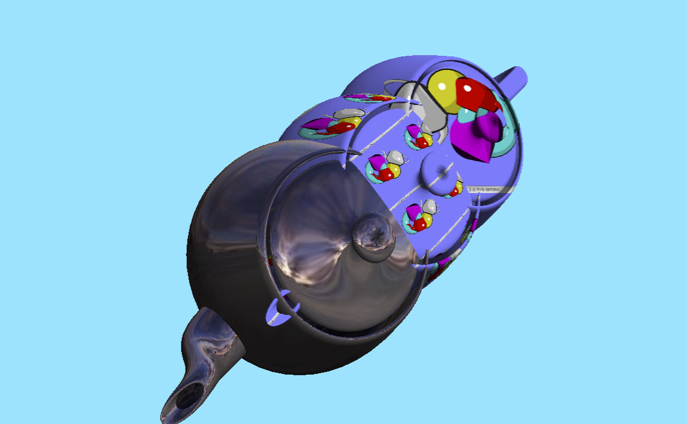
\includegraphics[width=9cm]{OGL_texture/mappingComparison2.png} 
	\end{tabular}
    \caption{텍스처 좌표 자동 생성 기법의 비교}
    \label{fig:OGL_texture:mappingComparison}
\end{figure}

\section{다중 텍스처}

지금까지는 하나의 물체에 하나의 텍스처만을 입혔다. 그런데, 필요에 따라 다수의 텍스처를 하나의 물체에 적용해야할 경우도 있다. 본 절에서는 이러한 다중 텍스처 적용에 대해 다룰 것이다.

\subsection{텍스처 매핑 유니트}
\index{texture!mapping unit}
\index{texture mapping unit}
\index{텍스처!매핑 유니트}
\index{텍스처 매핑 유니트}

우선 텍스처 매핑 유니트(unit)에 대해서 이해하자. 텍스처 매핑 유니트는 TMU라 줄여서 표현하기도 한다. 이것은 그래픽 처리 장치(GPU)의 부분 요소로서 전통적으로는 분리된 물리적 프로세스였다. 각각의 TMU는 3차원 객체의 임의 평면에 이미지 비트맵(bitmap)을 회전하거나 크기조정하여 부착할 수 있는 기능을 가지고 있다. 현대의 그래픽 카드에서는 이 유니트들이 그래픽스 파이프라인 상에서 서로 다른 단계(stage)로 구현되어 있다. 하나의 물체에 여러 개의 텍스처를 입히는 작업은 하나의 객체를 그릴 때에 여러 개의 텍스처 매핑 유니트를 거치는 일이 된다. 따라서 텍스처 이미지를 읽고 텍스처를 준비하는 작업을 여러 개의 유니트, 혹은 단계(stage)에 따로 따로 이루어지게 된다.
OpenGL에서는 텍스처 매핑과 관련된 함수들이 어떠한 유니트에 적용되는지를 지정할 수 있는 API가 제공되는데, 이것이 {\sf glActiveTexture}이다. 만약 {\sf glActiveTexture(GL\_TEXTURE0)}가 호출되면, 이후의 모든 텍스처 작업은 텍스처 유니트 0번에서 이뤄지는 일이 된다. 간단한 예를 통해 이 텍스처 유니트를 이해해 보자.


\subsection{다중 텍스처 연습}
\index{다중 텍스처}
\index{multitexture}
\index{texture!multitexture}
\index{텍스처!다중 텍스처}

주전자 표면에 고정된 텍스처를 입히고, 주변환경을 반사하는 텍스처도 함께 붙이는 것을 통해 다중 텍스처링과 텍스처 매핑 유니트에 대해 이해해 보자.
텍스처를 읽어들이는 함수는 앞에서 살펴본 것과 동일한 코드를 사용한다. 주전자 표면에 부착된 텍스처 이미지와, 반사되는 환경을 표현하는 구면 맵 텍스처 이미지를 읽어야 한다. 
우선 다음 그림 \ref{fig:OGL_texture:multiTex}과 같은 두 종류의 텍스처를 준비한다.

\begin{figure}[h!]
  \centering
	\begin{tabular}{cc}
	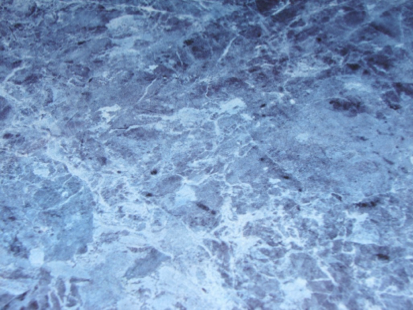
\includegraphics[height=6cm]{OGL_texture/multiTex_A.png} &
	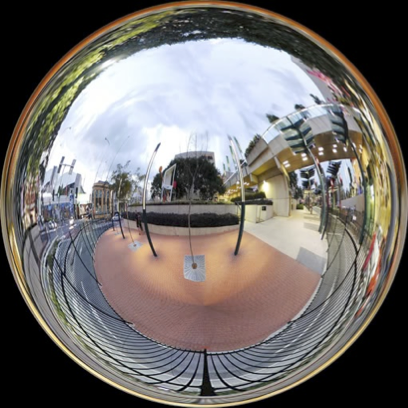
\includegraphics[height=6cm]{OGL_texture/multiTex_B.png}  \\
	{\sf \small (a) 텍스처 A (surface.jpg)} & {\sf \small (b) 텍스처 B (spheremap.jpg)}
	\end{tabular}
    \caption{다중 텍스처 매핑에 사용될 두 개의 텍스처 이미지}
    \label{fig:OGL_texture:multiTex}
\end{figure}

이 두 텍스처를 읽어들이는 것은 앞에서 살펴본 {\sf texture.h/cpp}의 {\sf setTexture} 함수를 사용하면 된다. 그런데, {\sf surface.jpg}는 텍스처 매핑 유니트 0에, 
{\sf spheremap.jpg}는 텍스처 매핑 유니트 1의 텍스처로 할당하려고 한다. 이것은 {\sf glActiveTexture} 함수를 사용하여 구현할 수 있다. 
구체적인 구현 방법은 다음 코드 \ref{code:textureUnit}와 같다.

\begin{algorithmbis}[두 개의 텍스처를 읽어 각각 0, 1 텍스처 유니트에 할당]\label{code:textureUnit}
\lstset{language=C++, escapechar=^} 
\begin{lstlisting}
// filename: main.cpp

void init(int argc, char **argv) {
  initWindow(&argc, argv);
  ...
  // ^{\it 텍스처 유니트 0에 텍스처를 하나 할당}^
  glActiveTexture(GL_TEXTURE0);
  tex1 = setTexture("surface.jpg");

  // ^{\it 텍스처 유니트 1에 텍스처를 하나 할당}^
  glActiveTexture(GL_TEXTURE1);
  tex2 = setTexture("spheremap.jpg");

  LightSet();
  glEnable(GL_DEPTH_TEST);
}
\end{lstlisting}
\end{algorithmbis}

그림을 그릴 때는 코드 \ref{code:multiTexture}와 같은 방식을 사용한다.
이 코드를 사용하면, 구면 맵은 텍스처 좌표가 자동으로 생성되게 하고, 표면에 부착되는 텍스처는 주전자 그리기 함수에서 주어진 텍스처 좌표를 그대로 사용한다.

\begin{algorithmbis}[두 장의 텍스처가 모두 매핑된 주전자 그리기]\label{code:multiTexture}
\lstset{language=C++} 
\begin{lstlisting}
    glEnable(GL_TEXTURE_2D);
    glActiveTexture(GL_TEXTURE0);
    glBindTexture(GL_TEXTURE_2D, tex1);
    glActiveTexture(GL_TEXTURE1);
    glBindTexture(GL_TEXTURE_2D, tex2);
    glEnable(GL_TEXTURE_GEN_S);  glEnable(GL_TEXTURE_GEN_T);
    glTexGenf(GL_S, GL_TEXTURE_GEN_MODE,  GL_SPHERE_MAP);
    glTexGenf(GL_T, GL_TEXTURE_GEN_MODE,  GL_SPHERE_MAP);
    glutSolidTeapot(1.2);
    glDisable(GL_TEXTURE_GEN_S);  glDisable(GL_TEXTURE_GEN_T);
\end{lstlisting}
\end{algorithmbis}

\begin{figure}[h!]
  \centering
	\begin{tabular}{cc}
	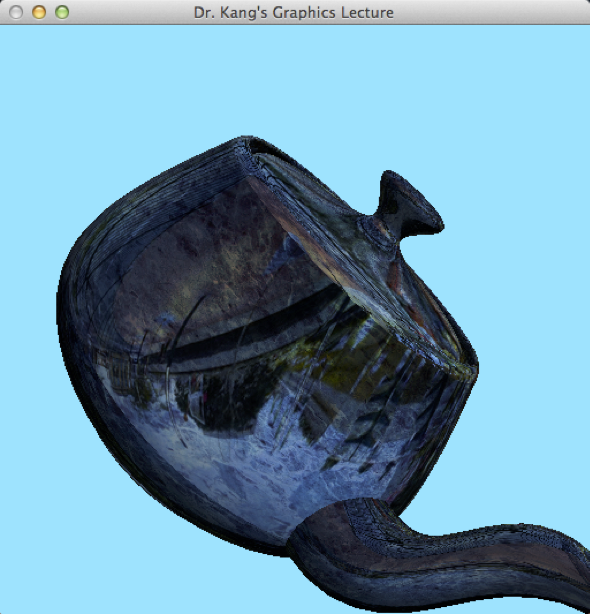
\includegraphics[height=6cm]{OGL_texture/multiTexturedA.png} &
	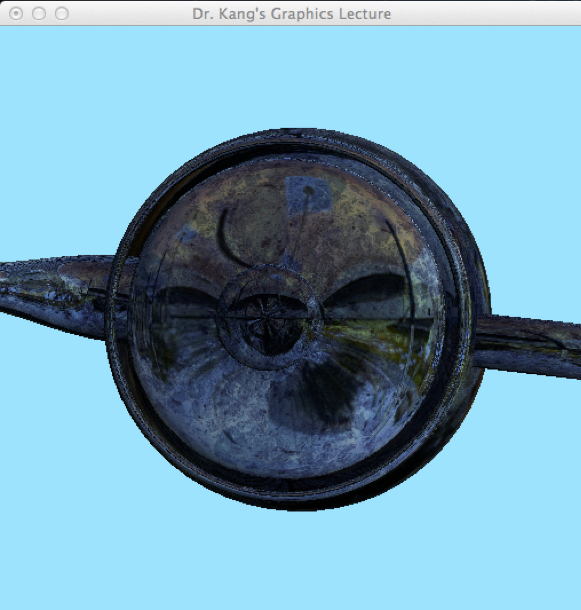
\includegraphics[height=6cm]{OGL_texture/multiTexturedB.png}  \\
	\end{tabular}
    \caption{구면 매핑 기법을 통해 두 장의 이미지를 주전자에 입힌 결과}
    \label{fig:OGL_texture:multiTextured}
\end{figure}

코드 \ref{code:multiTexture}와 같은 방법으로 그리면, 텍스처 매핑 유니트 1에 해당하는 구면 맵에 대해서 구면 맵에 사용되는 텍스처 좌표가 자동으로 결정된다. 텍스처 유니트 0에 있는 텍스처는 따로 텍스처 좌표 자동 생성을 적용하지 않았기 때문에 정점의 속정으로 주어진 텍스처 좌표에 따라 {\sf surface.jpg}의 이미지가 주전자 표면에 붙게 된다.
이상과 같은 코드의 렌더링의 결과는 그림 \ref{fig:OGL_texture:multiTextured}과 같다.



다음으로는 텍스처 좌표를 직접 변경하는 작업을 수행해 볼 것이다.
텍스처를 읽는 것은 앞의 예와 동일하다. 이번에는 한장의 사각형 평면을 그리자. 그리고 0번 유니트의 텍스처와 1번 유니트의 텍스처에 서로 다른 텍스처 좌표를 부여한다.
이번에는 텍스처를 다음 그림 \ref{fig:OGL_texture:multiTex2}에 나타난 것들을 사용하자.

\begin{figure}[h!]
  \centering
	\begin{tabular}{cc}
	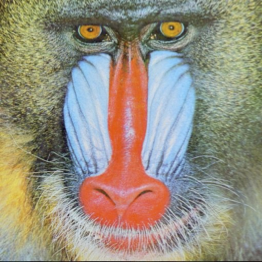
\includegraphics[height=6cm]{OGL_texture/multiTex2A.png} &
	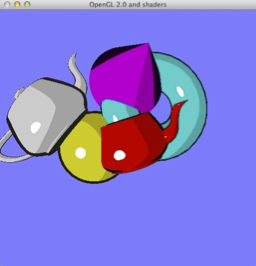
\includegraphics[height=6cm]{OGL_texture/multiTex2B.png}  \\
	\end{tabular}
    \caption{다중 텍스처 매핑에 사용될 새로운 두 이미지}
    \label{fig:OGL_texture:multiTex2}
\end{figure}

이 두 장의 텍스처 이미지를 서로 다른 텍스처 좌표를 이용하여 매핑하는 방법은 다음 코드
\ref{code:multiTex2}처럼 구현할 수 있다.

\begin{algorithmbis}[텍스처 두 장의 텍스처 좌표를 명시적으로 달리 설정하는 법]\label{code:multiTex2}
\lstset{language=C++} 
\begin{lstlisting}
	glBegin(GL_QUADS);
	glNormal3f(0.0, 0.0, 1.0);
	glMultiTexCoord2f(GL_TEXTURE0, 0.0, 0.0);
	glMultiTexCoord2f(GL_TEXTURE1, 0.0, 0.0);
	glVertex3f(-0.5, 0.5, 0.0);
	glMultiTexCoord2f(GL_TEXTURE0, 0.0, 1.0);
	glMultiTexCoord2f(GL_TEXTURE1, 0.0, 2.0);
	glVertex3f(-0.5,-0.5, 0.0);
	glMultiTexCoord2f(GL_TEXTURE0, 1.0, 1.0);
	glMultiTexCoord2f(GL_TEXTURE1, 2.0, 2.0);
	glVertex3f( 0.5,-0.5, 0.0);
	glMultiTexCoord2f(GL_TEXTURE0, 1.0, 0.0);
	glMultiTexCoord2f(GL_TEXTURE1, 2.0, 0.0);
	glVertex3f( 0.5, 0.5, 0.0);
	glEnd();
\end{lstlisting}
\end{algorithmbis}

결과는 다음과 같이 원숭이 얼굴 그림은 화면 전체에 하나가 그려지지만, 카툰 렌더링 결과 이미지는 네 번 나타난다.
\begin{figure}[h!]
  \centering
	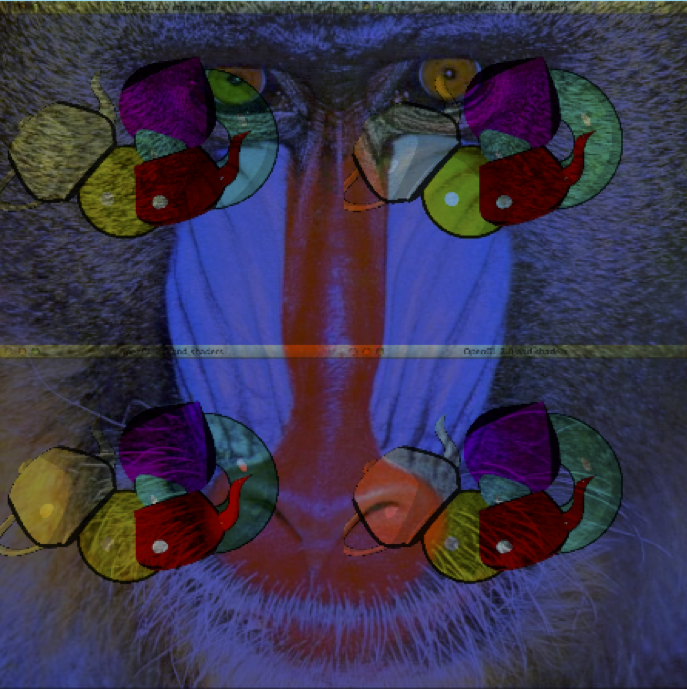
\includegraphics[height=6cm]{OGL_texture/multiTex2.png} 
    \caption{텍스처 두 장의 텍스처 좌표를 명시적으로 달리 설정한 결과}
    \label{fig:OGL_texture:multiTex2}
\end{figure}

\section{텍스처 좌표의 변환과 텍스처 애니메이션}
\index{texture!coordinate transform}
\index{텍스처!좌표 변환}
\index{texture coordinate transform}
\index{텍스처 좌표 변환}

텍스처 좌표 역시 객체의 위치를 결정하는 기하 좌표처럼 변환을 적용할 수 있다. 우리가 앞서 살펴본 행렬 모드는 {\sf GL\_MODELVIEW}와 {\sf GL\_PROJECTION}의 두 종류였다. 우리가 사용하지 않은 행렬 모드로 {\sf GL\_TEXTURE} 행렬이 있는데, 이 행렬은 텍스처 좌표를 변환하는 데에 사용된다. 이 절에서는 이 모드를 활용하여 텍스처 좌표를 변환하는 방법을 살펴볼 것이다.

\subsection{텍스처 좌표 변환}
텍스처 좌표를 변환하기 위해서는 {\sf glMatrixMode}을 사용하여 조작하는 행렬이 {\sf GL\_TEXTURE}임을 밝혀야 한다. 
우선 간단한 크기변경부터 시작해 보자. 우선 다음 그림 \ref{fig:OGL_texture:multiTex3}과 같은 텍스처를 준비한다.

\begin{figure}[h!]
  \centering
	\begin{tabular}{cc}
	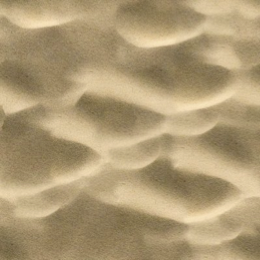
\includegraphics[height=4cm]{OGL_texture/terrain.png} &
	
\includegraphics[height=4cm]{OGL_texture/science.png}  \\
	{\sf \small (a) 텍스처 A (terrain.jpg)} & {\sf \small (b) 텍스처 B (science.jpg)}
	\end{tabular}
    \caption{다중 텍스처 애니메이션에 사용될 두 개의 텍스처 이미지}
    \label{fig:OGL_texture:multiTex3}
\end{figure}

우선 두 텍스처를 앞의 다중 텍스처 매핑 기법을 이용하여 다음 코드 \ref{code:multiTexForAnimation}과 같이 겹쳐 보이도록 하자.
결과는 그림 \ref{fig:OGL_texture:multiTexForAni}와 같다.

\begin{algorithmbis}[두 장의 텍스처에 동일한 텍스처 좌표 설정]\label{code:multiTexForAnimation}
\lstset{language=C++} 
\begin{lstlisting}
glBegin(GL_QUADS);
glMultiTexCoord2f(GL_TEXTURE0, 0.0, 0.0);
glMultiTexCoord2f(GL_TEXTURE1, 0.0, 0.0);
glVertex3f(-0.5, 0.5, 0.0);
glMultiTexCoord2f(GL_TEXTURE0, 0.0, 1.0);
glMultiTexCoord2f(GL_TEXTURE1, 0.0, 1.0);
glVertex3f(-0.5,-0.5, 0.0);
glMultiTexCoord2f(GL_TEXTURE0, 1.0, 1.0);
glMultiTexCoord2f(GL_TEXTURE1, 1.0, 1.0);
glVertex3f( 0.5,-0.5, 0.0);
glMultiTexCoord2f(GL_TEXTURE0, 1.0, 0.0);
glMultiTexCoord2f(GL_TEXTURE1, 1.0, 0.0);
glVertex3f( 0.5, 0.5, 0.0);
glEnd();
\end{lstlisting}
\end{algorithmbis}

\begin{figure}[h!]
  \centering
	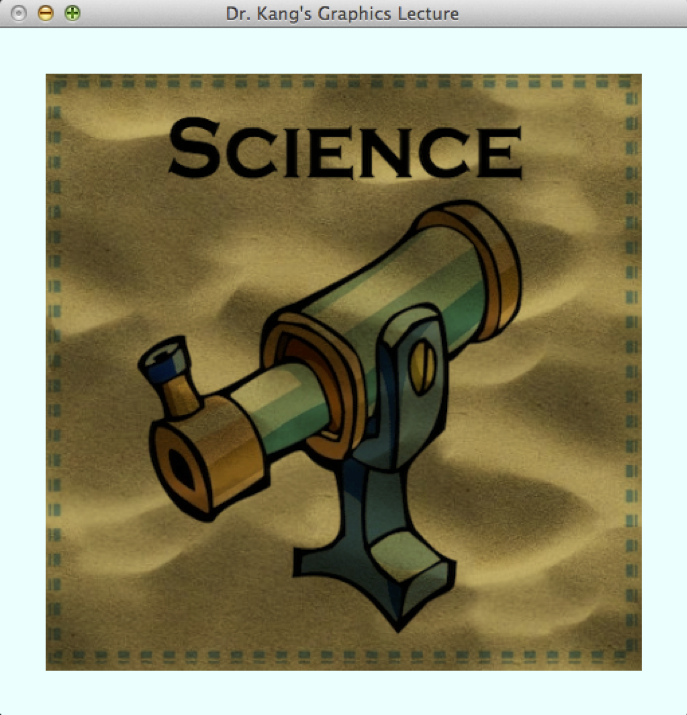
\includegraphics[height=6cm]{OGL_texture/multiTexForAni.png} 
    \caption{애니메이션 될 두 텍스처를 동시에 매핑한 결과}
    \label{fig:OGL_texture:multiTexForAni}
\end{figure}

이제 두 번째 텍스처({\sf GL\_TEXTURE1})이 사각형 면에 한 번이 아니고 축소된 형태로 여러번 반복하여 나타나게 하여 보자. 
이러기 위해서는 두 번째 텍스처 유니트에 적용되는 좌표를 수작업으로 변경하는 방법이 있다. 이는 바로 앞 절에서 사용한 방식이다. 
이 절에서는 텍스처 좌표를 변환하는 방식을 사용한다. 따라서 {\sf glScale*} 함수를 사용할 것이다. 이를 위해서 다음 코드 \ref{code:multiTexXform}와 같이 고친다.
지금까지 우리는 {\sf glMatrixMode}를 이용하여 행렬 보드를 {\sf GL\_PROJECTION}이나 {\sf GL\_MODELVIEW} 모드로 변경하는 일은
빈번히 해 왔다. 이와 같은 방법으로 텍스처에 적용되는 좌표 변환 행렬 모드를 설정할 수 있다. 이를 위해서는 행렬 모드를 {\sf GL\_TEXTURE}로 지정한다.
\begin{algorithmbis}[텍스처 좌표를 변환하기]\label{code:multiTexXform}
\lstset{language=C++, escapechar=^} 
\begin{lstlisting}
    glActiveTexture(GL_TEXTURE0);
    glBindTexture(GL_TEXTURE_2D, tex1);
    glActiveTexture(GL_TEXTURE1);
    glBindTexture(GL_TEXTURE_2D, tex2);
    ^{\bf \color{red} glMatrixMode(GL\_TEXTURE)}^; //^{\it 행렬 모드를 텍스처 모드로 바꾼다}^
    glLoadIdentity();
    glScalef(5.0, 5.0, 1.0);    
    glBegin(GL_QUADS);
    ^{\sf 코드 \ref{code:multiTexForAnimation}와 같은 내용으로 작성}^
    glEnd();
\end{lstlisting}
\end{algorithmbis}

실행 결과는 그림 \ref{fig:OGL_texture:multiTexturedForAni}와 같다.

\begin{figure}[h!]
    \centering
	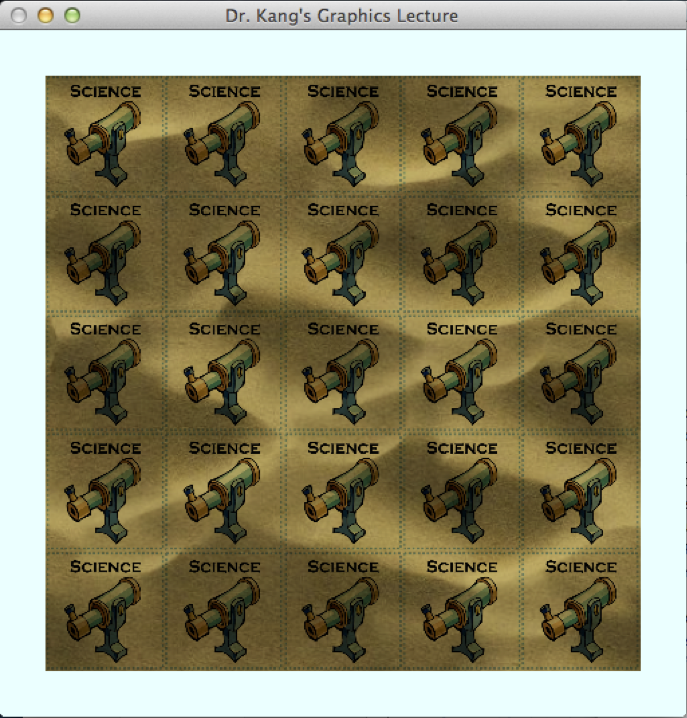
\includegraphics[height=6cm]{OGL_texture/multiTexturedForAni.png} 
    \caption{유니트 별로 다르게 설정된 텍스처 변환 행렬}
    \label{fig:OGL_texture:multiTexturedForAni}
\end{figure}

그림 \ref{fig:OGL_texture:multiTexturedForAni}에서 볼 수 있는 바와 같이 특정한 텍스처 유니트에 대해 텍스처 좌표를 변환하는 작업이 가능하다는 것이다. 이를 이용하여 텍스처 좌표를 프레임마다 변경하는 텍스처 애니메이션도 구현할 수 있다.

\index{texture!animation}
\index{texture animation}
\index{텍스처 애니메이션}
\index{텍스처!애니메이션}

다음 코드는 텍스처 유니트 0에 있는 {\sf terrain.jpg}는 크기가 커졌다가 작아지는 일을 반복하게 하고, 
텍스처 유니트 1에 있는 {\sf science.jpg}는 왼쪽으로 흘러가도록 만들어 보겠다.
구현은 코드 \ref{code:multiTexAnimation}에 있으며,
그 수행 결과는 그림 \ref{fig:OGL_texture:multiTexAnimation}에 나타나 있다.

\begin{algorithmbis}[두 장의 텍스처에 서로 다른 애니메이션 변환 적용]\label{code:multiTexAnimation}
\lstset{language=C++} 
\begin{lstlisting}
glActiveTexture(GL_TEXTURE0);
glMatrixMode(GL_TEXTURE);
glLoadIdentity();
glScalef(1.0+sin(t)*0.1, 1.0+sin(t)*0.1, 1.0);
	
glActiveTexture(GL_TEXTURE1);
glMatrixMode(GL_TEXTURE);
glLoadIdentity();
glTranslatef(t,0,0);
glScalef(5.0, 5.0, 1.0);
glEnd();
\end{lstlisting}
\end{algorithmbis}

이상의 코드를 실행하면 다음과 같이 0번 유니트의 텍스처는 크기가 커졌다 줄었다 하며, 
1번 유니트의 텍스처는  5분의 1 크기로 줄어서 부착되며, 계속해서 $x$축 음의 방향으로 이동한다.
결과는 그림 \ref{fig:OGL_texture:multiTexAnimation}에 나타나 있다.

\begin{figure}[h!]
    \centering
	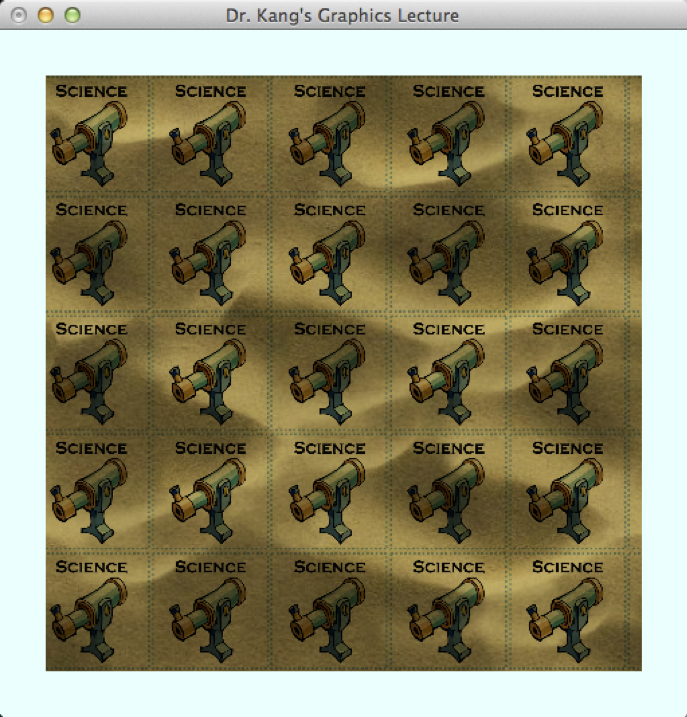
\includegraphics[height=6cm]{OGL_texture/multiTexAni_A.png} 
	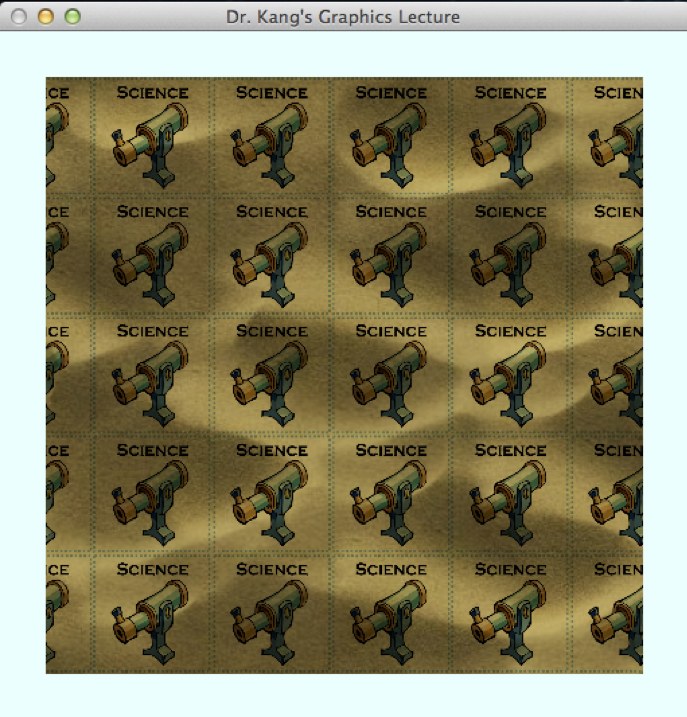
\includegraphics[height=6cm]{OGL_texture/multiTexAni_B.png} 
    \caption{다중 텍스처의 애니메이션}
    \label{fig:OGL_texture:multiTexAnimation}
\end{figure}

텍스처 매핑과 관련된 다양한 이론과 기술들에 대한 깊은 이해를 위해서는 \cite{hearn1997computer,akenine2011real,foley1994introduction}와 같은 여러 그래픽스 교재를 참고하라.
